\section{ML vs DL}

\subsection{Feature Extraction}

In beiden Fällen unterlaufen die Daten den selben Phasen: Feature Extraction und Classification. Jedoch unterscheiden sie sich bei der Ausführung der Feature Extraction.

In der Feature Extraction werden Merkmale zusammengefasst und in einer strukturierten Tabelle dargestellt. Jede Zeile beinhaltet diese Merkmale und die dazugehörige Klassifizierung.

Bei einem \gls{ml}-Modell ist die Feature Extraction ein separater Vorgang, welcher nicht automatisch durch das Modell vorgenommen wird. Dieser Prozess ist oft sehr kompliziert und beansprucht eine lange Zeit, außerdem ist hier eine Person notwendig, die sich in dem gegebenen Bereich auskennt.

Im Kontrast dazu nutzt ein \gls{dl}-Modell ein Neuronales Netzwerke, welches sich stark an einem menschlichen Gehirn orientiert und die Feature Extraction übernimmt.

\begin{figure}[H]
    \centering
    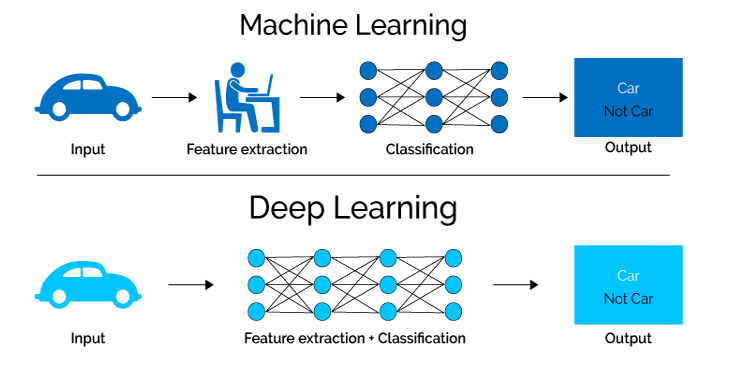
\includegraphics[scale=0.6]{sections/machine-learning/images/MLvsDL.png}
    \caption{Feature Extraction, ML vs DL}
\end{figure}

Wie der Name ''Neuronales Netzwerk'' vorschlagt, besteht dieses Konzept aus tausenden nachgeahmten Neuronen, die über mehrere Schichten zusammen kommunizieren. Dabei kann sich ein Neuron nur mit anderen Neuronen auf der selben oder darüberlegenden Schicht verknüpfen, daher entsteht eine hierarchische Struktur.

Die einzelnen Schichten können mit den fünf Sinnen eines Menschen verglichen werden. Verbindet man zum Beispiel einer Person die Augen und lässt sie dann eine Erdbeere probieren, kann die Person anhand des Geschmackes und des Duftes erkennen, um welche Frucht es sich handelt. Ähnlich würde es in einem Neuronalen Netzwerk ablaufen, wobei der Geschmack und der Duft einzelne Schichten repräsentieren.

Legt die Person daraufhin die Augenbinde ab und sieht, dass die Erdbeere weiß, kann sie sich trotzdem sicher sein, dass es sich um eine Erdbeere handel, da sie aus Erfahrung sagen kann, dass der Geschmack und Duft eindeutiger sind. Dies würde ein Neuronales Netzwerk am Anfang verwirren, da es nicht über diese Erfahrung verfügt. Mit der Zeit würde das Neuronale Netzwerk bestimmten Synapsen (Verbindungen) eine Gewichtung zuteilen, welche die Wichtigkeit einzelner Parameter angibt. Dieses Einordnen ist die Art, wie ein Neuronales Netzwerk ''lernt''.\cite{NN}

\subsection{Vergleich}

Ein \gls{ml}-Modell sollte bevorzugt in Bereichen genutzt werden, wo bereits strukturierte Daten vorhanden sind. Die Menge an Daten ist hierbei nicht sehr relevant, da ein \gls{ml}-Modell mit wenigen Daten präzise sein kann.

Stehen keine bereits vorpräparierte Daten zur Verfügung, wäre ein \gls{dl}-Modell die bessere Lösung, da man sich die Zeit und Kosten für die Feature Extraction sparen kann. Jedoch benötigt man leistungsstarke Computer, da Neuronale Netzwerke komplexe Rechnungen durchführen, die mithilfe einer GPU beschleunigt werden können. Außerdem ist die Programmierung und Trainingsphase sehr lang und mühselig. \cite{MLvsDL}

Bei der Entscheidung welches Modell sinnvoller ist, sollte man außerdem beachten, dass die Technologie noch nicht voll entwickelt ist und dass manche Probleme mit dem momentanen Stand der Technik nicht lösbar sind.